%%%%%%%%%%%%%%%%%%%%%%%%%%%%%%%%%%%%%
%Presentazione esame di Dottorato Davide Spataro
%result.tex
%Purpose: Contains the results of the benchmarks of both opencal and opencal-cluster. 
% for each tests it shows graphs and table when available and also comment them.
%@author Davide Spataro
%@version 1.0 14/01/2018 Eindhoven
%%%%%%%%%%%%%%%%%%%%%%%%%%%%%%%%%%%%

\section[Computational Results]{Validation and Computational Results}
\frame{\frametitle{Benchmarks} 
	\begin{block}{3 performance tests adopted}
		\begin{itemize}
			\item Julia Set Generation $\Longrightarrow$ \textbf{compute} bound 
			\item Convolutional Filtering $\Longrightarrow$ \textbf{memory} bound
			\item \texttt{sciddicaT} landslide model $\Longrightarrow$ \textbf{compute}+\textbf{memory} bound
		\end{itemize}
	\end{block}
\pause
\begin{block}{Test HW}
	\begin{itemize}
		\item up to $4$ nodes interconnected via GigaBit Ethernet 
		\item up to $8$ GPUs: GTX980, K40,K20 and Tesla 2090
	\end{itemize}
\end{block}
}

\subsection{Julia Set}
\frame{\frametitle{Julia Set - Algorithm} 
	\begin{itemize}
		\item $z_0 = x + yi$ with $x$ and $y$ pixel coordinate is initilized
		\item $z$ is repeatedly updated using: $z_{n+1} = f(z_n)$
		\item in our case $f(z_n)= z_n^2 + c$
		\item if $z_k$ is lower than a threshold then $(x,y)$ belongs to the set and is pictured in white. If it does, then a color is assigned  with shade depending on $k$.
	\end{itemize}
	\begin{figure}
	\centering
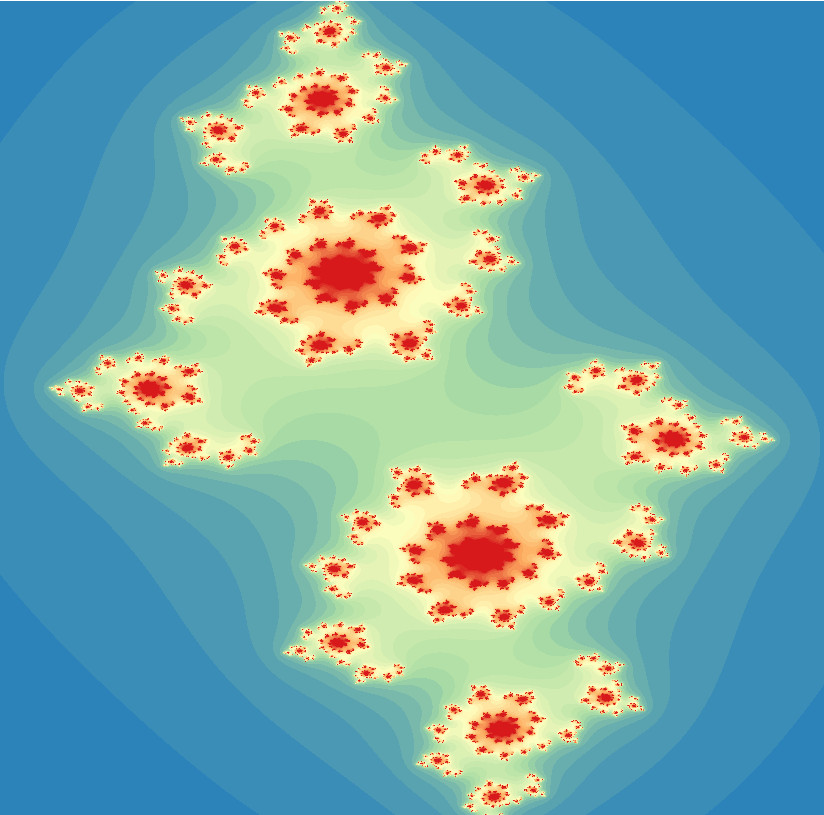
\includegraphics[scale=0.2]{./images/fractal16k16k}
\end{figure}
 
}

%\frame{\frametitle{Julia Set - multi-GPU speedup} 
%	\begin{figure}
%	\centering
%	\includegraphics[width=0.55\textwidth]{images/fractal_false_scaling}
%	\caption{Julia set speedups obtained on single-GPU execution (K40 ,GTX980) and	multi-GPU execution on two devices ($144 \times 10^6$ grid points).}
%\end{figure}
%}

\frame{\frametitle{Julia Set - multinode/multi-GPU speedup} 
	\begin{columns}
		\begin{column}{0.48\textwidth}
			\begin{figure}
				\centering
					\includegraphics[width=1\textwidth]{images/fractal_false_scaling}
			\end{figure}
		\end{column}
		\begin{column}{0.48\textwidth}
			\begin{figure}
				\centering
				\includegraphics[width=1\textwidth]{images/fractal_direnzo_scaling}
				%\caption{Gaussian Blur Filter}
				%\caption{Julia set speedups obtained on single-GPU execution (K40 ,GTX980) and	multi-GPU execution on two devices ($144 \times 10^6$ grid points).}
			\end{figure}
		\end{column}
	\end{columns}
	\begin{itemize}
		\item domain sizes $225\times10^6$(left),$484\times10^6$(right) grid points
		\item \#\texttt{instruction Sobel} $\approx$ $2$\#\texttt{instruction Blur}
		\item GTX980 faster on memory bound code
	\end{itemize}
	
}



\frame{\frametitle{Julia Set - K40 vs GTX980} 

	\begin{figure}
		\centering
		\includegraphics[width=1\textwidth]{images/fractal12k_k40_980_true}
		\caption{Time and Speed-up for the Julia Set case ($1200 \times 10^6$ grid points) on two different GPUs: 1
			GTX980 and 1 K40 . The bottom and top horizontal axes indicate the amount of rows assigned to the K40 and GTX980 , respectively.}
	\end{figure}
}


\subsection{Convolutional Filtering}
\frame{\frametitle{Convolutional Filtering} 
	\begin{itemize}
		\item Very common in image processing 
		\item The value of the grid point is substituted with a weighted average of neighboring points
		\item Little floating-point computation involved $\Longrightarrow$ memory bound
\end{itemize}
\begin{figure}
	\centering
	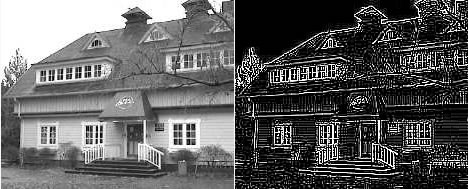
\includegraphics[scale=0.55]{./images/sobel_example}
	\caption{Sobel Convolutional Filtering Example}
\end{figure}
}

\frame{\frametitle{Convolutional Filtering} 
	2D convolution can be formalized as follows:
	\begin{equation*}
	f'_{ij} = \sum_{i'=0}^n \sum_{j'=0}^m f_{(i+i')(j+j')}\times d_{ij}
	\label{eq:convolution}
	\end{equation*}
	where 
	\begin{itemize}
		\item $m,n$ are the  vertical and horizontal size of the kernel,
		\item $f_{ij}$ and $f'_{ij}$ are the old and new value of the cell at coordinate $(i,j)$,
		\item $d_{ij}$ is the value of kernel (weights) at location $(i,j)$ 
	\end{itemize}
	\begin{figure}
		\centering
		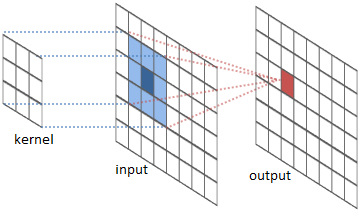
\includegraphics[scale=0.68]{./images/conv_illustration}
	\end{figure}
}


\frame{\frametitle{Sobel/Gaussian Filters - multi-GPU speedup} 
	\begin{columns}
		\begin{column}{0.48\textwidth}
				\begin{figure}
				\centering
				\includegraphics[width=0.95\textwidth]{images/sobel_scaling}
				\caption{Sobel Filter}
			%	\caption{Julia set speedups obtained on single-GPU execution (K40 ,GTX980) and	multi-GPU execution on two devices ($144 \times 10^6$ grid points).}
			\end{figure}
		\end{column}
		\begin{column}{0.48\textwidth}
				\begin{figure}
				\centering
				\includegraphics[width=0.95\textwidth]{images/blur_scaling}
				\caption{Gaussian Blur Filter}
				%\caption{Julia set speedups obtained on single-GPU execution (K40 ,GTX980) and	multi-GPU execution on two devices ($144 \times 10^6$ grid points).}
			\end{figure}
		\end{column}
	\end{columns}
\begin{itemize}
	\item domain size $= 225\times10^6$ grid points
	\item \#\texttt{instruction Sobel} $\approx$ $2$\#\texttt{instruction Blur}
	\item GTX980 faster on memory bound code
\end{itemize}

}

\frame{\frametitle{Sobel Filter - K40 vs GTX980} 
	
	\begin{figure}
		\centering
		\includegraphics[width=1\textwidth]{images/sobel_2nodes_k40_980}
		\caption{K40 vs GTX980 on two nodes interconnected via GigaBit Ethernet.}
	\end{figure}
}




\subsection{sciddicaT - debris flow simulation CA}
\frame{\frametitle{sciddicaT model} 
	\begin{itemize}
		\item Features \textit{memory/compute} and \textit{memory\&compute} bound kernels
		\item Simulations of real events e.g. \textit{Tessina  landslide}
		\item Flows distribution via \textit{differences minimization algorithm}\footnote{S. D. Gregorio, R. Serra, \textit{An empirical method for modelling and simulating some complex macroscopic phenomena by cellular automata}, 1999.}
	\end{itemize}
	\begin{figure}
		\centering
		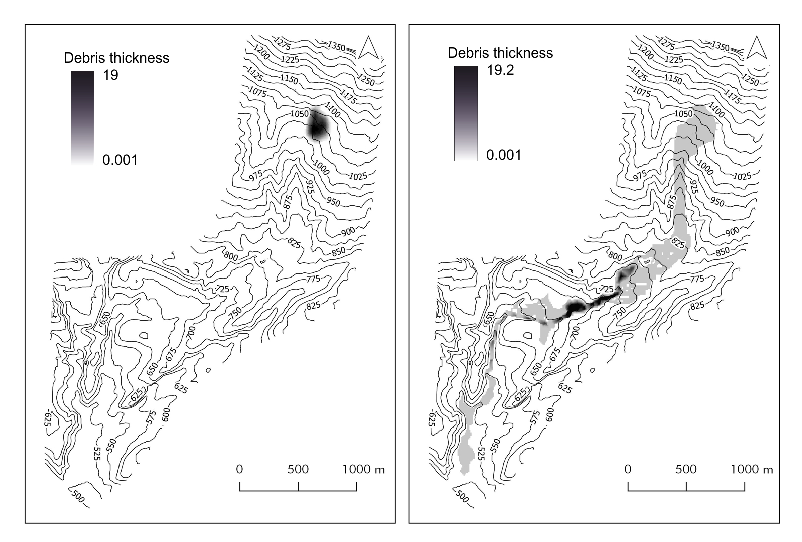
\includegraphics[scale=0.55]{./images/Figure05_new}
	\end{figure}
}

\frame{\frametitle{Shared Memory - Built-in Optimizations} 
\hfill \\
\centering
\textbf{domain size = $610 \times 496$ grid cells}
	\begin{figure}
	\centering
	\includegraphics[width=\textwidth]{./images/Figure07_new-eps-converted-to}
\end{figure}
}

\frame{\frametitle{Shared Memory - Built-in Optimizations} 
	\hfill \\
	\centering
	\textbf{domain size = $3593 \times 3730$ grid cells}
	\begin{figure}
		\centering
		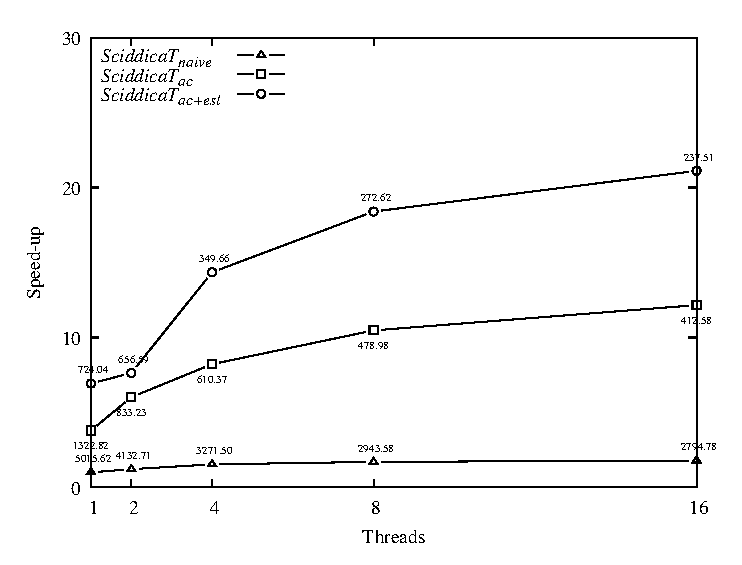
\includegraphics[width=\textwidth]{./images/Figure12_new}
	\end{figure}
}



\frame{\frametitle{multi-GPU} 
	\begin{columns}
	\begin{column}{0.48\textwidth}
		\begin{figure}
			\centering
			\includegraphics[width=1\textwidth]{images/sciddicaT_standard_scaling}
			\caption{$610 \times 496$ grid cells}
		\end{figure}
	\end{column}
	\begin{column}{0.48\textwidth}
		\begin{figure}
			\centering
			\includegraphics[width=1\textwidth]{images/sciddicaT_scaling}
			\caption{ $3593 \times 3730$ grid cells}
		\end{figure}
	\end{column}
\end{columns}

}

